% Z -> tau_h tau_h cross section with CMS Open Data -- methods, choices, findings.
% Build (from z-tautau/):  python slides/make_figures.py && cd slides && pdflatex ztautau_slides.tex (twice)
% Needs beamer + metropolis; the texlive in /data/atlas/users/nterlind lacks translator.sty and pgfopts.sty:
% unpack them from CTAN (translator.zip, pgfopts.tds.zip) somewhere and export TEXINPUTS=".:<dir>//:".
% Figures: ../output/plots/*.pdf|png (scripts/step3,4,6) and fig_*.pdf (make_figures.py).
\documentclass[aspectratio=169,9pt]{beamer}
\usetheme[progressbar=frametitle,numbering=fraction]{metropolis}
\usepackage{booktabs}
\usepackage{tikz}
\usetikzlibrary{positioning,arrows.meta,shapes.misc}
\usepackage{graphicx}
\usepackage{amsmath}
\graphicspath{{../output/plots/}{./}}
\definecolor{tau}{HTML}{D9822B}
\definecolor{fake}{HTML}{E377AC}
\definecolor{mc}{HTML}{4A90D9}
\setbeamercolor{frametitle}{bg=black!85}
\setbeamercolor{progress bar}{fg=tau}
\setbeamercolor{alerted text}{fg=tau!90!black}
\newcommand{\tauh}{\ensuremath{\tau_\mathrm{h}}}
\newcommand{\mtt}{\ensuremath{m_{\tau\tau}}}
\newcommand{\mvis}{\ensuremath{m_\mathrm{vis}}}
\setlength{\tabcolsep}{4pt}
\setbeamertemplate{frametitle}{\nointerlineskip\begin{beamercolorbox}[wd=\paperwidth,leftskip=0.3cm,sep=0.18cm]{frametitle}\usebeamerfont{frametitle}\insertframetitle\end{beamercolorbox}}

\title{$\mathbf{Z\rightarrow\tau_h\tau_h}$ cross section with CMS Open Data}
\subtitle{Methods, choices and findings}
\author{BND School 2026 -- Z$\rightarrow\tau\tau$ subgroup}
\date{14 September 2026 \quad\textbullet\quad branch \texttt{z-tautau}}

\begin{document}

\maketitle

% -----------------------------------------------------------------------------------------------
\begin{frame}{The measurement at a glance}
\begin{columns}[T]
\begin{column}{0.53\textwidth}
\small
\textbf{Goal:} $\sigma(pp\rightarrow Z/\gamma^*\rightarrow\tau\tau)$ with both $\tau$ decaying hadronically, in the same
TRExFitter framework as $ee$ and $\mu\mu$, ready for a combined fit.

\medskip
\textbf{Data:} CMS 2016 \texttt{Tau} dataset, Run2016G+H (UL NanoAODv9), 156\,M events,
$L = 16.39\,\mathrm{fb}^{-1}$ (normtag, same in all channels)

\medskip
\textbf{Strategy}
\begin{itemize}\setlength\itemsep{1pt}
\item two \tauh{} ($p_T>40$\,GeV), OS, DeepTau Medium: 47\,586 events
\item \alert{81\,\% jet$\rightarrow$\tauh{} fakes} $\Rightarrow$ fake factor from data, no QCD MC
\item Z$\rightarrow\tau\tau$ + small backgrounds from UL16 simulation, TauPOG corrections
\item MET folded into the visible mass: likelihood mass \mtt
\item binned profile-likelihood fit of \mtt, TRExFitter v1.8.0 (shared binary)
\end{itemize}
\end{column}
\begin{column}{0.45\textwidth}
\centering
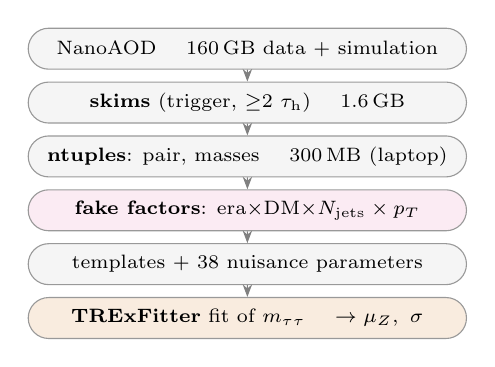
\begin{tikzpicture}[node distance=1.5mm, every node/.style={font=\scriptsize, rounded rectangle, draw=black!40, fill=black!4, minimum width=5.8cm, minimum height=5.2mm}, >={Stealth[length=1.6mm]}]
\node (a) {NanoAOD \quad 160\,GB data + simulation};
\node (b) [below=of a] {\textbf{skims} (trigger, $\geq$2 \tauh) \quad 1.6\,GB};
\node (c) [below=of b] {\textbf{ntuples}: pair, masses \quad 300\,MB (laptop)};
\node (d) [below=of c, fill=fake!15] {\textbf{fake factors}: era$\times$DM$\times N_\mathrm{jets}\times p_T$};
\node (e) [below=of d] {templates + 38 nuisance parameters};
\node (f) [below=of e, fill=tau!15] {\textbf{TRExFitter} fit of \mtt{} \quad $\rightarrow\mu_Z,\ \sigma$};
\foreach \x/\y in {a/b,b/c,c/d,d/e,e/f} \draw[->, black!50] (\x) -- (\y);
\end{tikzpicture}

\vspace{2mm}
\begin{beamercolorbox}[rounded=true, shadow=false, sep=4pt]{block body}
\small
$\sigma(Z/\gamma^*\!\rightarrow\!\tau\tau,\,60\text{--}120) = 2255\pm36\,^{+371}_{-315}\pm83$\,pb\\
NNLO: 1945\,pb \qquad $\mu_Z = 1.16\,^{+0.19}_{-0.16}$
\end{beamercolorbox}
\end{column}
\end{columns}
\end{frame}

% -----------------------------------------------------------------------------------------------
\begin{frame}{Selection: choices and why}
\begin{columns}[T]
\begin{column}{0.58\textwidth}
\footnotesize
\begin{tabular}{@{}p{2.2cm}p{5.6cm}@{}}
\toprule
trigger & \texttt{DoubleMedium(Combined)IsoPFTau35\_Trk1\_eta2p1\_Reg}: G has only \emph{Iso}, H only \emph{CombinedIso}; both legs matched to HLT $\tau$ objects \\
\tauh{} & $p_T>40$ (plateau side of the 35\,GeV leg), $|\eta|<2.1$, DM 0/1/10/11 (calibrated modes) \\
DeepTau 2017v2p1 & VSe VVLoose, VS$\mu$ VLoose; \textbf{VSjet Medium} = tight, VVVLoose$\wedge\neg$Medium = loose \\
pair & most isolated, $\Delta R>0.5$; $\tau_1$ = leading $p_T$ (FF leg) \\
vetoes & no extra $e$/$\mu$: orthogonal to $e\tau_h$, $\mu\tau_h$, $ee$, $\mu\mu$ \\
simulation & drop events whose \textbf{leading $\tau$ is a jet} (covered by the FF) \\
\bottomrule
\end{tabular}
\end{column}
\begin{column}{0.40\textwidth}
\footnotesize
\begin{tabular}{@{}lrr@{}}
\toprule
cutflow & Run2016G & Run2016H \\
\midrule
NanoAOD & 79.6\,M & 76.8\,M \\
skim & 2.81\,M & 2.22\,M \\
pair + MET filters & 2.03\,M & 1.62\,M \\
trigger match & 1.99\,M & 1.59\,M \\
lepton veto & 1.99\,M & 1.59\,M \\
\textbf{SR} (OS, Medium) & \textbf{24\,106} & \textbf{23\,480} \\
\bottomrule
\end{tabular}

\medskip
\textbf{Expected SR composition}\\
fakes 38\,746 \quad Z$\rightarrow\tau\tau$ 7\,878\\
$t\bar t$ 570, W+jets 514, Z$\rightarrow ee$ 208, VV 122

\medskip
\alert{Signal acceptance is tiny:} $A = 0.23\,\%$\\ (B$_{hh}\approx42\,\%$ $\times$ both visible $\tau$ above 40\,GeV)
\end{column}
\end{columns}
\end{frame}

% -----------------------------------------------------------------------------------------------
\begin{frame}{MET correction of the visible di-$\tau$ mass}
\begin{columns}[T]
\begin{column}{0.40\textwidth}
\footnotesize
$\geq4$ neutrinos escape: \mvis{} peaks at $0.8\,m_Z$.
\begin{itemize}\setlength\itemsep{2pt}
\item \textbf{collinear approx.}: solve MET $=\sum_i(1/x_i-1)\,\vec p_{T,i}^{\,vis}$\\
singular for back-to-back $\tau$: \alert{defined in 38\,\%}
\item \textbf{likelihood mass \mtt} (FastMTT/SVfit-lite idea): scan $(x_1,x_2)$ on a grid,\\
weight $=\exp(-\tfrac12 r^TV^{-1}r)$ {\scriptsize(MET covariance)}\\
\phantom{weight} $\times$ flat 2-body phase space $\times\,1/m^2$\\
$\rightarrow$ posterior median, always defined
\end{itemize}
\footnotesize
\begin{tabular}{@{}lcc@{}}
\toprule
 & scale & resolution \\
\midrule
\mvis & 0.80 & 13\,\% \\
\mtt{} (used) & \textbf{0.99} & \textbf{11\,\%} \\
\bottomrule
\end{tabular}\\[1mm]
{\scriptsize Z$\rightarrow\tau\tau$/fakes in the best window: 2.6 (\mtt) vs 2.3 (\mvis)}
\end{column}
\begin{column}{0.31\textwidth}
\centering
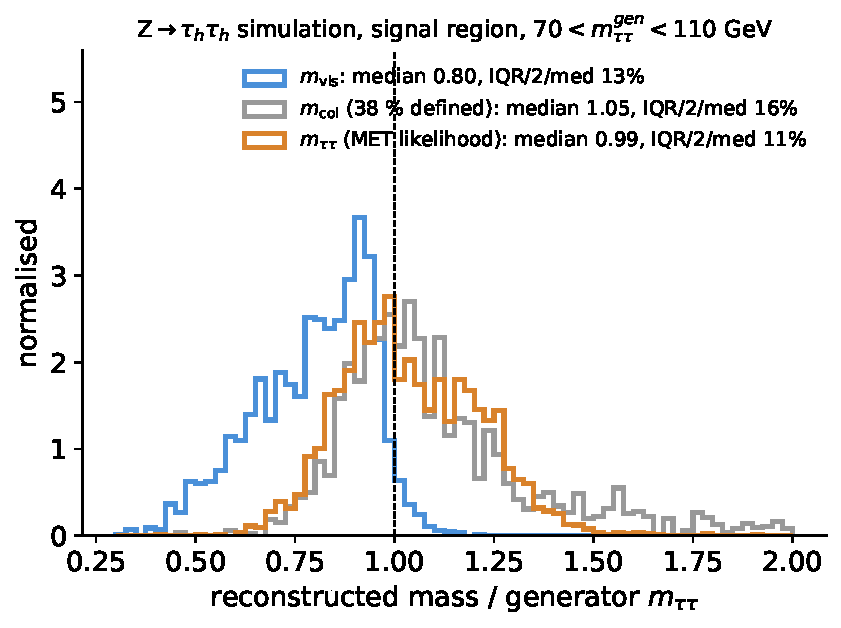
\includegraphics[width=\linewidth]{fig_mass_estimators.pdf}\\[1mm]
\scriptsize Finding: correct scale and better resolution; separation power vs fakes about equal.
With $p_T>40$ on both legs the selected $\tau$ are already hard.
\end{column}
\begin{column}{0.29\textwidth}
\centering
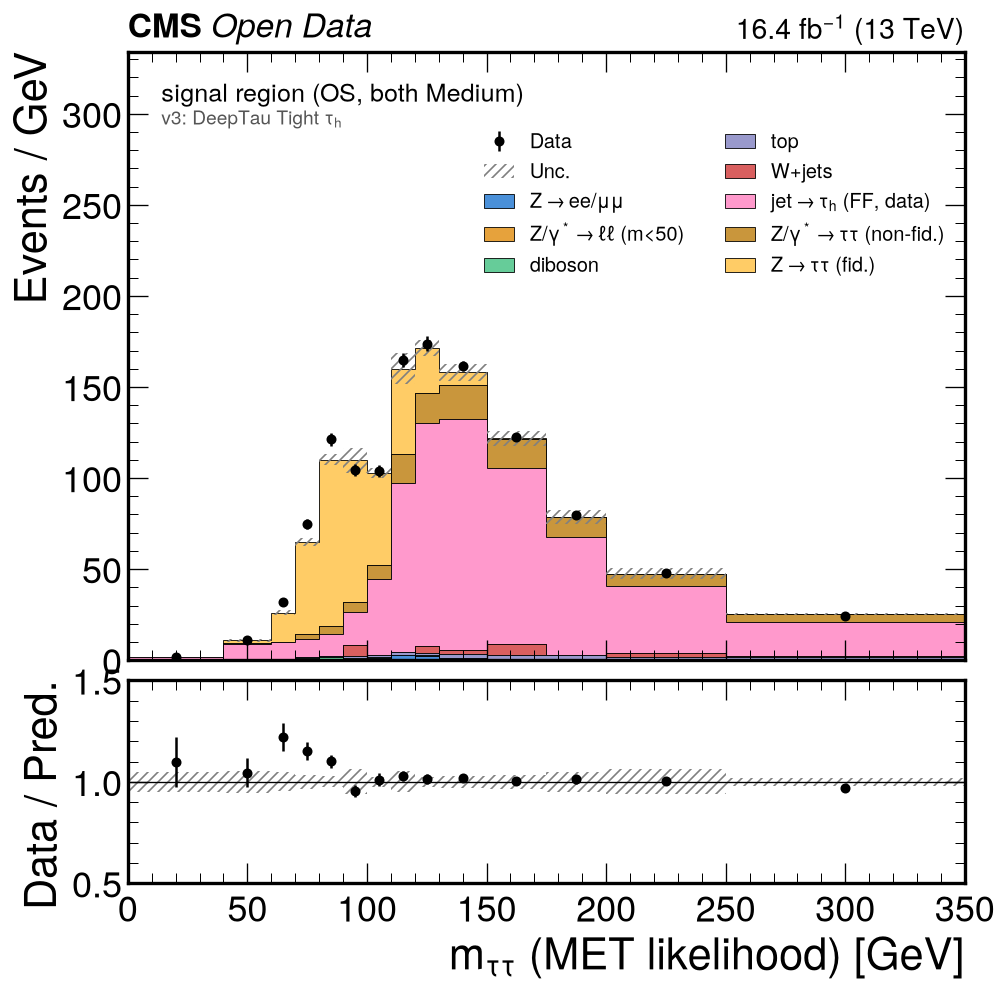
\includegraphics[width=\linewidth]{step4_SR_m_tt.pdf}\\
\scriptsize Signal region, prefit: Z peak at $m_Z$, fakes at 130--300\,GeV give the normalisation sideband.
\end{column}
\end{columns}
\end{frame}

% -----------------------------------------------------------------------------------------------
\begin{frame}{Jet$\rightarrow\tau_h$ fakes: the classic fake factor}
\begin{columns}[T]
\begin{column}{0.50\textwidth}
\small
\[
\mathrm{FF} = \frac{N(\text{SS},\ \tau_1\ \text{Medium},\ \tau_2\ \text{Medium})}{N(\text{SS},\ \tau_1\ \text{VVVL}\wedge\neg\text{M},\ \tau_2\ \text{Medium})}
\]
\[
N_\text{fake}^\text{SR} = \sum_{\text{OS},\ \tau_1\neg\text{M},\ \tau_2\text{M}} C_{OS/SS}\cdot\mathrm{FF}
\]
\vspace{-3mm}
\begin{itemize}\setlength\itemsep{1pt}
\item same-sign = QCD enriched (no Z); $\tau_2$ Medium in both $\Rightarrow$ isolation correlation absorbed
\item binning chosen by \textbf{closure} in same-sign data:
  \begin{itemize}\scriptsize
  \item $N_\mathrm{jets}$: off by $+9\,\%\ldots-25\,\%$ (quark/gluon mix)
  \item era: $-4\,\%$ (G) / $+5\,\%$ (H): different HLT $\tau$ isolation
  \end{itemize}
\item final: era $\times$ DM $\times$ $N_\mathrm{jets}$ (0,1,$\geq$2) $\times$ $p_T$ = 120 bins, $\sim$10\,\% stat.\ each
\item $C_{OS/SS}$ = 1.07--1.13 from the $\tau_2$ anti-isolated sideband, +3\,\% extrapolation syst.
\end{itemize}
\end{column}
\begin{column}{0.50\textwidth}
\centering
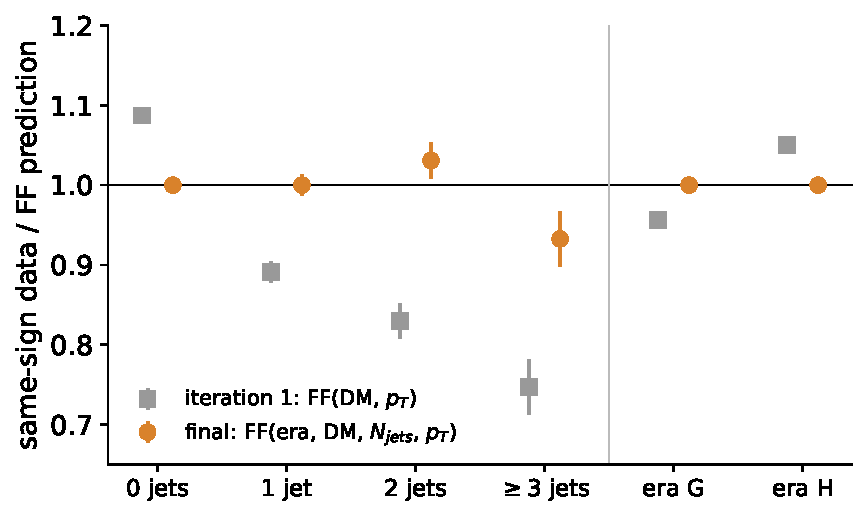
\includegraphics[width=0.74\linewidth]{fig_ff_closure.pdf}\\[0.5mm]
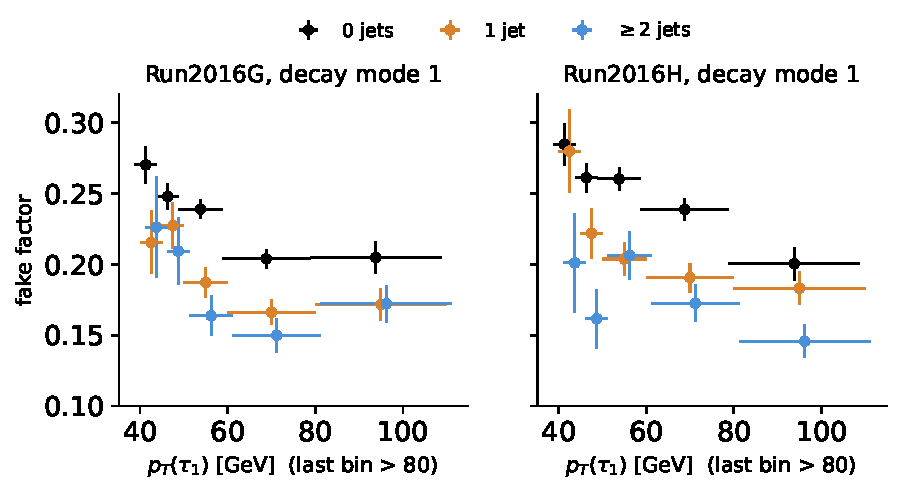
\includegraphics[width=0.88\linewidth]{fig_ff_dm1.pdf}\\
\scriptsize all 120 bins: \texttt{output/plots/step3\_fakefactors.png}
\end{column}
\end{columns}
\end{frame}

% -----------------------------------------------------------------------------------------------
\begin{frame}{The MC-subtraction question}
\begin{columns}[T]
\begin{column}{0.56\textwidth}
\small
Genuine $\tau$ leak into the fake-factor regions (simulated, genuine $\tau_1$):\\[1mm]
\footnotesize
\begin{tabular}{@{}lrrr@{}}
\toprule
region & data & genuine $\tau_1$ & fraction \\
\midrule
SS, $\tau_1$ Medium (FF num.) & 26\,761 & 232 & 0.9\,\% \\
OS, $\tau_1$ fails (application) & 187\,973 & 2\,386 & 1.3\,\% \\
OS, $\tau_2$ anti-iso ($C$ num.) & 219\,737 & 8\,321 & 3.8\,\% \\
\bottomrule
\end{tabular}

\medskip\small
\begin{itemize}\setlength\itemsep{2pt}
\item \textbf{Nominal (as specified): no subtraction.} Signal is double counted in the application region and $C$ is biased up.
\item Alternative ``mcsub'' computed everywhere: prefit fakes $-4.5\,\%$ = \alert{22\,\% of the signal}; $C$: 1.078$\rightarrow$1.051
\item But post-fit: $\mu_Z$ = 1.160 vs 1.208 --- the high-\mtt{} sideband re-normalises the fakes (\texttt{FakeOSSS} pulled $-0.86\sigma$ towards mcsub)
\item \textbf{Recommendation:} make ``mcsub'' nominal next
\end{itemize}
\end{column}
\begin{column}{0.42\textwidth}
\centering
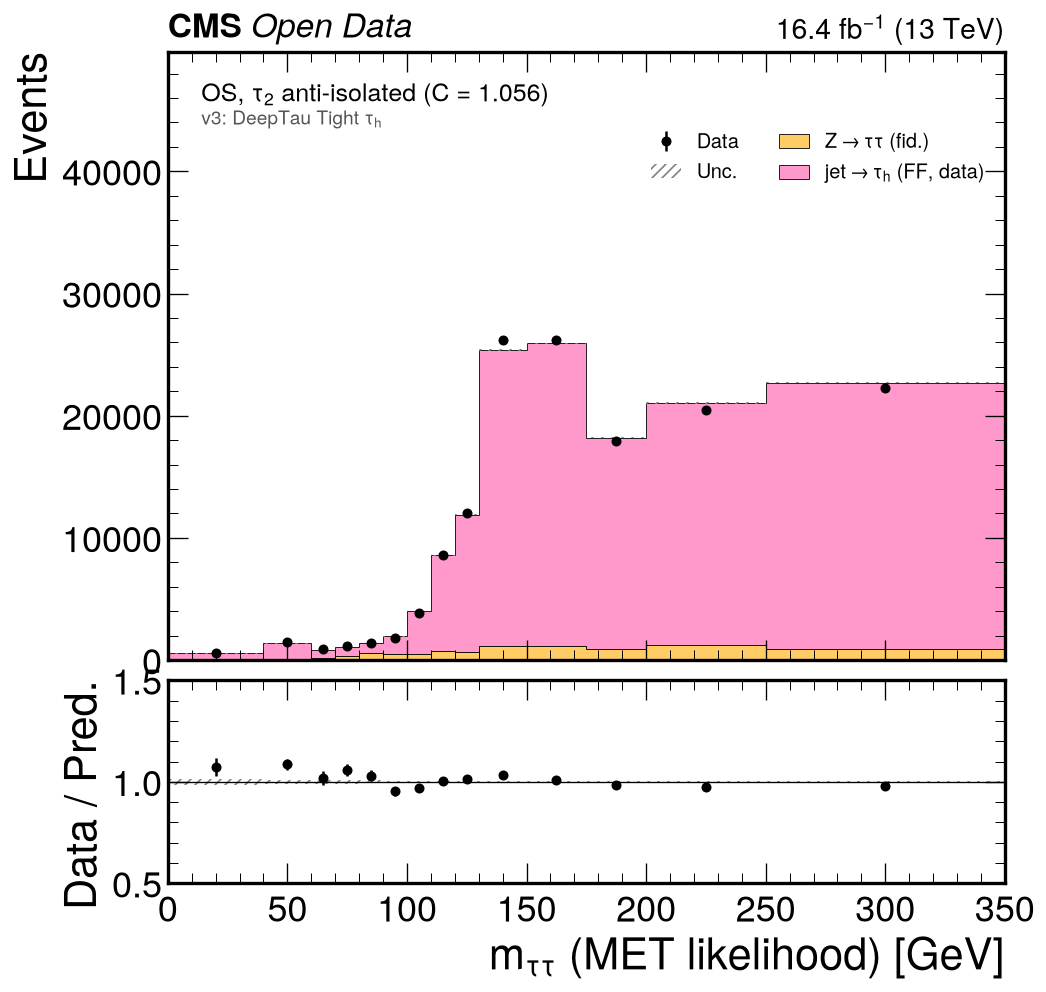
\includegraphics[width=0.92\linewidth]{step3_OSAI_m_tt_mcsub.pdf}\\
\scriptsize OS, $\tau_2$ anti-isolated: after $C$ and subtraction the SS$\rightarrow$OS shape closes within $\pm5\,\%$.
\end{column}
\end{columns}
\end{frame}

% -----------------------------------------------------------------------------------------------
\begin{frame}{Simulation, corrections and systematic uncertainties}
\begin{columns}[T]
\begin{column}{0.52\textwidth}
\footnotesize
\textbf{TauPOG UL2016 postVFP} (public GitHub; cvmfs/GitLab not reachable)\\[1mm]
\begin{tabular}{@{}lcccc@{}}
\toprule
 & DM0 & DM1 & DM10 & DM11 \\
\midrule
ID SF (Medium) & 0.92(14) & 0.88(5) & 0.87(9) & 0.90(16) \\
energy scale & 0.993(9) & 0.991(7) & 1.001(7) & 0.997(16) \\
trigger SF @50 & 0.94(5) & 0.97(4) & 0.94(5) & 1.07(8) \\
\bottomrule
\end{tabular}\\[1mm]
+ e/$\mu\rightarrow\tau_h$ SFs, pileup (Open Data lumi table), L1 prefiring

\medskip
\textbf{38 nuisance parameters + 14 $\gamma$}, names shared across channels:\\
\texttt{Lumi, Pileup, L1Prefiring, QCDScale, PDF, PS\_ISR/FSR, SigModel} (correlated);
\texttt{TauID/Trigger/ES\_DM*}, \texttt{MET\_Unclustered}, \texttt{Fake*\_tautau}, \texttt{XS\_*}
\end{column}
\begin{column}{0.46\textwidth}
\small
\textbf{Choices that mattered}
\begin{itemize}\setlength\itemsep{2pt}
\item theory variations \emph{renormalised to the fiducial yield}: only $C$ in the fit, $A$ separate (3.7\,\%)
\item LO vs NLO generator: normalisation only ($\Delta C = 7.3\,\%$)
\item W+jets: few events, weights up to $\sim$200 $\Rightarrow$ shape from $\tau_2\geq$VVVLoose, 50\,\% norm.\ NP
\end{itemize}
\textbf{Bugs found and fixed}
\begin{itemize}\setlength\itemsep{2pt}\footnotesize
\item scale envelope \& PDF Hessian taken \emph{per event}: $\pm15\,\%$ / $\pm4\,\%$ $\rightarrow$ per histogram: $\pm4\,\%$ / $\pm1\,\%$ \quad ($\sigma_\mu$: 26\,\%$\rightarrow$18\,\%)
\item forked worker pools deadlock after uproot; uproot $\geq$5.6 writes dicts as RNTuple
\end{itemize}
\end{column}
\end{columns}
\end{frame}

% -----------------------------------------------------------------------------------------------
\begin{frame}{The fit}
\begin{columns}[T]
\begin{column}{0.36\textwidth}
\centering
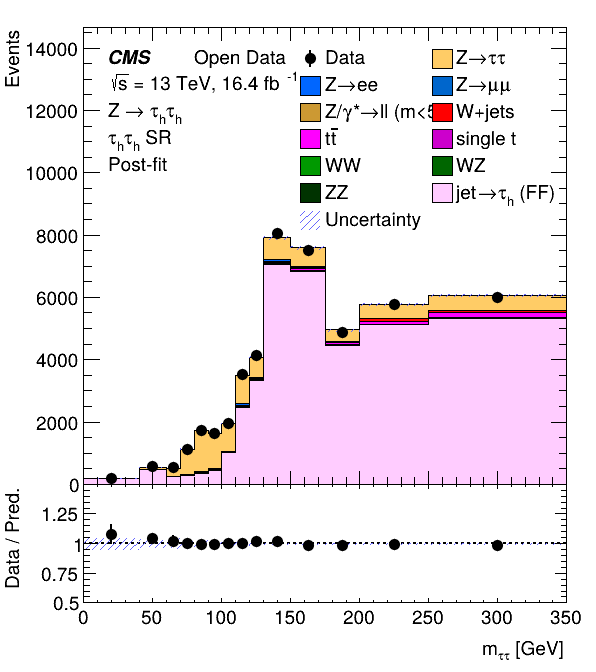
\includegraphics[width=\linewidth]{fit_SR_postfit.png}\\
\scriptsize post-fit \mtt{} in the SR; GoF $p = 0.18$
\end{column}
\begin{column}{0.34\textwidth}
\centering

\includegraphics[width=\linewidth]{fit_ranking.png}
\end{column}
\begin{column}{0.28\textwidth}
\footnotesize
\small
\begin{itemize}\setlength\itemsep{2pt}
\item one region, 14 bins of \mtt{} (0--350\,GeV)
\item $\mu_Z$ on Z$\rightarrow\tau\tau$; fakes from data with FF nuisances
\item bins above 130\,GeV (95\,\% fakes) fix the fake normalisation: post-fit fakes $-2.8\,\%$
\item pulls within $1\sigma$; \texttt{FakeClosure} constrained to 0.32
\item uncertainty on $\mu_Z$:\\ expected $^{+0.169}_{-0.140}$, observed $^{+0.192}_{-0.163}$
\item stat-only: $\pm0.018$
\end{itemize}
\end{column}
\end{columns}
\end{frame}

% -----------------------------------------------------------------------------------------------
\begin{frame}{Result}
\begin{columns}[T]
\begin{column}{0.52\textwidth}
\centering

\includegraphics[width=\linewidth]{step6_summary.pdf}\\[2mm]
\small
\begin{tabular}{@{}lr@{}}
\toprule
$\sigma(Z/\gamma^*\!\rightarrow\!\tau\tau,\ 60<m<120)$ & $2255\pm36\,^{+371}_{-315}\pm83_{A}$\,pb \\
\quad prediction (FEWZ NNLO) & 1945\,pb \\
$\sigma_\mathrm{fid}(\tau_h\tau_h$, $p_T^{vis}>40$, $|\eta|<2.1)$ & $5.22\pm0.08\pm0.80$\,pb \\
\quad prediction & 4.50\,pb \\
$\mu_Z$ (nominal / mcsub) & $1.160^{+0.192}_{-0.163}$ / $1.208^{+0.201}_{-0.169}$ \\
\bottomrule
\end{tabular}
\end{column}
\begin{column}{0.46\textwidth}
\centering
\vspace{3mm}
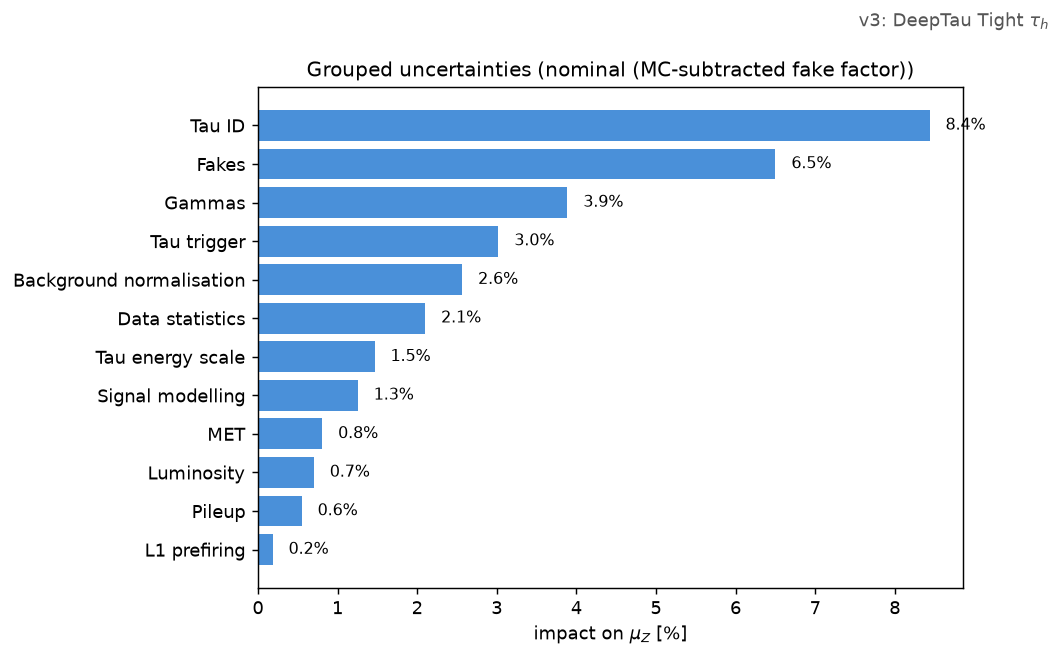
\includegraphics[width=\linewidth]{step6_impacts.pdf}\\
\scriptsize grouped impacts on $\mu_Z$ (nominal)
\end{column}
\end{columns}
\end{frame}

% -----------------------------------------------------------------------------------------------
\begin{frame}{Findings and next steps}
\begin{columns}[T]
\begin{column}{0.52\textwidth}
\textbf{Findings}
\small
\begin{enumerate}\setlength\itemsep{2pt}
\item Consistent with NNLO within $1\sigma$; data statistics 1.8\,\%, total $^{+17}_{-14}\,\%$.
\item \alert{The limit is external}: TauPOG \tauh{} ID SFs (12.5\,\%) --- Z$\rightarrow\tau\tau$ is how those SFs are measured.
\item Background is 5$\times$ the signal; only a \emph{shape} fit works (counting: 1815\,pb, driven by a 3\,\% fake normalisation).
\item The FF needs $N_\mathrm{jets}$ and era binning to close; the MC-subtraction choice moves prefit fakes by 22\,\% of the signal but $\mu_Z$ by only 4\,\%.
\item The MET-likelihood mass fixes the scale and improves the resolution, but does not add discrimination at $p_T>40$.
\end{enumerate}
\end{column}
\begin{column}{0.46\textwidth}
\textbf{For the combination}
\small
\begin{itemize}\setlength\itemsep{1pt}
\item workspace \texttt{fit/results/ztautau}, POI \texttt{mu\_Z}: plugs into \texttt{fitting/combination\_skeleton.config}
\item with $ee/\mu\mu$ fixing $\mu_Z$, $\tau\tau$ constrains the \tauh{} ID NPs (lepton universality)
\end{itemize}
\textbf{Next steps}
\begin{itemize}\setlength\itemsep{1pt}
\item MC-subtracted FF as nominal; closure corrections in $\eta(\tau_1)$, $p_T(\tau_2)$
\item NLO-only signal-model prescription (LO vs NLO: 8.5\,\%)
\item more DY statistics (jet-binned), HT-binned W+jets
\item add $e\tau_h$/$\mu\tau_h$: \tauh{} ID in situ
\end{itemize}
\scriptsize Code, docs, handoff: \texttt{z-tautau/} (README, CLAUDE.md, docs/00--08)
\end{column}
\end{columns}
\end{frame}

\end{document}
